\PassOptionsToPackage{table}{xcolor} % load colortbl when xcolor is loaded - for coloring tables
\documentclass[10pt,twoside,sfsidenotes]{tufte-handout}

% --- Custom Preamble ---
%========================================
% Quiz Preamble
%========================================

%----------- Encoding and Fonts ----------
\usepackage[T1]{fontenc}
\usepackage[utf8]{inputenc}
\usepackage{bm}
\usepackage{mathrsfs}
\usepackage{siunitx}
\usepackage{amsmath}  
\usepackage{mathtools}

%----------- Document Layout -------------
\usepackage{geometry}
\geometry{bottom=0.5in, top=0.75in, left=0.75in, right=2.75in}
\usepackage{ragged2e}
\usepackage{multicol}
\usepackage{lipsum}

%----------- Exam/Exercises --------------
\usepackage{exsheets}
\SetupExSheets{
  question/type=exam,
  solution/print=false,
  headings=block-subtitle,
  counter-format=qu
}
\NewQuSolPair{sagequestion}[name={\sage Question}]{sagesolution}
\newcommand{\solspace}[1]{\examspace*{#1}}
%\renewcommand{\solspace}[1]{{\tiny\textsf{\textcolor{red}{Blank: #1}}}}

%----------- Graphics and Figures --------
\usepackage{graphicx}
  \setkeys{Gin}{width=\linewidth,totalheight=\textheight,keepaspectratio}
  \graphicspath{{./img/}} 
\usepackage{subcaption}
\captionsetup{compatibility=false}
\usepackage{pgfplots}
\usepackage{pgfplotstable}
\usepgfplotslibrary{patchplots}
\pgfplotsset{compat=newest}
\pgfplotstableset{row sep=crcr}

% Custom PGFPlots styles
\makeatletter
\pgfplotsset{
  tufte axes/.style = {
    after end axis/.code = {
      \draw ({rel axis cs:0,0} -| {axis cs:\pgfplots@data@xmin,0})
        -- ({rel axis cs:0,0} -| {axis cs:\pgfplots@data@xmax,0});
      \draw ({rel axis cs:0,0} |- {axis cs:0,\pgfplots@data@ymin})
        -- ({rel axis cs:0,0} -| {axis cs:0,\pgfplots@data@ymax});
    },
    axis line style = {draw = none},
    tick align      = outside,
    tick pos        = left
  },
  textbook axes/.style = {
    enlargelimits = true,
    axis line style = {->},
    axis lines = middle,
    axis x line=middle,
    tick align      = outside,
    tick pos        = left,
    y label style={at={(ticklabel* cs:1.05)}, anchor=south},
    x label style={at={(ticklabel* cs:1.05)}, anchor=west}
  },
  every axis/.append style = {
    mark size = 0pt,
    width=0.9\linewidth
  }
}
\makeatother

%----------- Tables ----------------------
\usepackage{booktabs}
\usepackage{units}

%----------- Code / Verbatim -------------
\usepackage{fancyvrb}
\fvset{fontsize=\normalsize}

%----------- Utilities -------------------
\usepackage{xspace}
\usepackage{etoolbox}
\usepackage{lastpage}
\usepackage{pdfpages}

%----------- Hyperlinks ------------------
\usepackage{url}
\usepackage{hyperref}
\hypersetup{
  bookmarksnumbered=true,
  colorlinks=true
}

%========================================
% Custom Commands and Environments
%========================================

% Month + Year
\newcommand{\monthyear}{%
  \ifcase\month\or January\or February\or March\or April\or May\or June\or
  July\or August\or September\or October\or November\or
  December\fi\space\number\year
}

% Column enumerate
\newenvironment{colenumerate}[1][2]
  {\begin{multicols}{#1}\begin{compactenum}[(a)]}
  {\end{compactenum}\end{multicols}}

% Empty grid
\newcommand{\emptygrid}[3][1.0]{%
  \def\width{#2}
  \def\hauteur{#3}
  \begin{tikzpicture}[x=10mm,y=10mm,semitransparent,scale=#1,every node/.style={scale=#1}]
    \draw[step=1mm, line width=0.1mm, black!30!white] (0,0) grid (\width,\hauteur);
    \draw[step=5mm, line width=0.2mm, black!40!white] (0,0) grid (\width,\hauteur);
    \draw[step=50mm, line width=0.5mm, black!50!white] (0,0) grid (\width,\hauteur);
    \draw[step=10mm, line width=0.3mm, black!90!white] (0,0) grid (\width,\hauteur);
  \end{tikzpicture}
}

% Section formatting (no chapter number)
\renewcommand*\thesection{\arabic{section}}
\setcounter{secnumdepth}{1}
\titleformat{\section}[hang]{\normalfont\large\bfseries}{\thesection}{0.5em}{}
\titleformat{\subsection}[hang]{\normalfont\bfseries}{\thesubsection}{0.5em}{}

% Math operators
\newcommand{\vv}[1]{\ensuremath{\underline{#1}}}
\newcommand{\mm}[1]{\ensuremath{\bm{#1}}}
\newcommand{\red}[1]{\textcolor{red}{#1}}
\DeclareMathOperator{\tr}{tr}
\DeclareMathOperator{\rank}{rank}
\DeclareMathOperator{\nullity}{nullity}
\let\Re\relax
\DeclareMathOperator{\Re}{\mathbb{R}e}
\let\Im\relax
\DeclareMathOperator{\Im}{\mathbb{I}m}
\DeclareMathOperator{\laplace}{\mathscr{L}}
\DeclareMathOperator{\hstep}{\mathscr{U}}

% Math delimiters
\DeclarePairedDelimiter{\norm}{\lVert}{\rVert}
\DeclarePairedDelimiter{\abs}{\lvert}{\rvert}
\DeclarePairedDelimiter{\iprod}{\langle}{\rangle}
\DeclarePairedDelimiter{\braced}\{\}

% Small bmatrix
\newenvironment{smallbmatrix}{\left[ \begin{smallmatrix*}[r]}{\end{smallmatrix*} \right]}

% Misc environments
\newenvironment{weekintro}{\begin{quote}}{\end{quote}}

% Handy macros
\newcommand{\sage}{\href{http://www.sagemath.org}{\textsf{\textsc{SageMath}}}\xspace}
\newcommand{\ode}{ODE\xspace}

% Roman numeral
\makeatletter
\newcommand*{\rom}[1]{\expandafter\@slowromancap\romannumeral #1@}
\makeatother

% Number equations within section
\numberwithin{equation}{section}
 % loads packages, custom commands, etc.

% Metadata
\date{} % suppress date
\SetVariations{2}
\variant{1}

% Fancy headers/footers
\fancyhead[L]{MATH 2860 -- E02 --- \monthyear}
\fancyhead[R]{\textbf{Name (Last, First):} \blank[width=3in]{}}
% \fancyhead[R]{\textbf{Name} (Last, First): \blank[width=3in]{} \\
% \textbf{Circle your TA}: Trevor \quad Yuchen \quad Samantha }
\fancyfoot[R]{\thepage/\pageref{LastPage}}




%----------------------------------------------------------
% --- Document ---
\begin{document}
\setlength\abovedisplayskip{2pt}
\setlength\belowdisplayskip{2pt}
\setlength\abovedisplayshortskip{2pt}
\setlength\belowdisplayshortskip{2pt}

\vspace*{1in}


   {\large I will not violate the University of Toledo Code of Ethics or assist others in doing so, especially by presenting others' work as mine, or allow them to present my work as theirs. \textbf{I am better than that} and I take pride in, and responsibility for, my work. I understand that violations of the Code may result in loss of credit for the exam, the course, or even jeopardize my academic standing.

\vspace{.5in}

    \textbf{Signed:}
  }

  \vfill


\begin{center}\Large
  \begin{tabular}{c | c | c}
    Problem & Max & Scored \\ \hline
     & & \\ \hline
     & & \\ \hline
     & & \\ \hline
     & & \\ \hline
     & & \\ \hline
     & & \\ \hline
     & & \\ \hline
     & & \\ \hline
    Exam grade & & \\ \hline
  \end{tabular}
  \end{center}

  \vfill

  \begin{fullwidth}
{\large
  \begin{itemize}
    \item Start the exam only at the proctor's signal.
%    \item The last page in this booklet is the \textbf{formula sheet}. Feel free to carefully detach it from the booklet.
  \item Closed books and notes, no brought-in summary sheets, formula sheets, or any such accessories.
  \item No external paper allowed; if you need extra paper, please ask the proctor for it.
  \item Only basic sci. calculators allowed; no graphing, matrix, or CAS calculators.
  \item If needed, use both sides of each sheet for your answers. Clearly indicate where the answer is written, if it is not in the space provided for it.
  \end{itemize}
  }
\end{fullwidth}
\clearpage


\begin{question}
  Given the ODE \marginnote{In all cases, use \textbf{real basis} (sines, cosines, etc.) where appropriate.}
  \[
    2\frac{d^{2}y}{dx^{2}} + 8 \frac{dy}{dx} + 8 y(x) = 0
  \]
  \begin{enumerate}[(a)]
    \item Calculate the general solution.
    
    \vfill

    \item Calculate the particular solution that satisfies \(y(0) = 4,\ y'(0) = 0\).

    \vfill
  \end{enumerate}
\end{question}

\clearpage
\begin{question}
    Find the general solution of the ODE: \marginnote{  In all cases, use \textbf{real basis} (sines, cosines, etc.) where appropriate. }
    \[
      \frac{d^{2}x}{dt^{2}} + 4x(t) = -16\,t + 4 +3 \sin(4t)
    \]
\end{question}

\clearpage
\begin{question}
  \begin{marginfigure}
    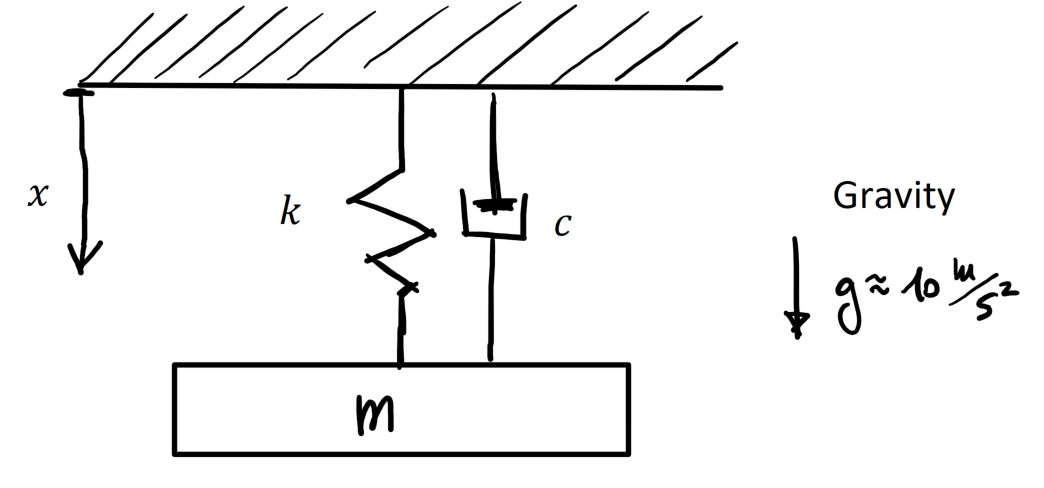
\includegraphics[width=\linewidth]{Exam_figs/rig.png}
  \end{marginfigure}
  A loading platform of mass \(m=10 \si{kg}\) that can move only along a vertical axis is supported by:
  \begin{compactitem}
    \item  a spring of undetermined spring constant \(k\), and
    \item a damper whose force is proportional to the speed at which it is being stretched or compressed with constant of proportionality \(c = 20 \si{N}\si{s}/\si{m}\).
  \end{compactitem}
   Take gravitational acceleration to be \(g \approx 10 \si{m}\si{s}^{-2}\).

  \begin{compactenum}[(a)]
    \item Determine the ODE for this mechanical system with undetermined \(k\). As needed, use free-body diagrams, force balance, etc.
    \item Calculate the value of \(k\) if you know that the platform sits at \(x_{EQ} = 1 \si{m}\) in the equilibrium (static) state.
    \item \marginnote{  In all cases, use \textbf{real basis} (sines, cosines, etc.) where appropriate. } Calculate the general solution for the motion of the platform.
    \item Sketch the solution \(x(t)\) that you calculated under (c) for an arbitrary non-equilibrium initial condition. Make sure your sketch demonstrates at least
      \begin{inparaenum}[(i)]
        \item presence/absence of oscillations,
        \item growth/decay of the amplitude, and 
        \item the limit as \(t\to\infty\).
      \end{inparaenum}
  \end{compactenum}
\end{question}

\clearpage
\begin{question}
  \begin{fullwidth}
    Explain: \textbf{What is resonance}, from physical and mathematical standpoints.

    \vspace{2in}

    What are the possible values of \(k\) in the equation below that result in resonance (\textbf{show your work}):
    \[
      2 \frac{d^{2}x}{dt^{2}} + 4 k x(t) = \sin(2t) + e^{3t}
    \]

    \vfill

    Form the \textbf{candidate for the forced solution} for the resonant case (that is, when \(k\) is set to the value in which resonance occurs). Show your work. (No need to find values of the coefficients, leave them as \(A,B,C,\dots\), just forming the candidate is enough.)

    \vfill

  \end{fullwidth}
\end{question}

\end{document}